\documentclass[a4paper,11pt]{book}
\usepackage{listings}
\usepackage{dirtree}
\usepackage[utf8]{inputenc}
\usepackage{titlesec}
\usepackage{fancyhdr}
\usepackage[spanish,es-tabla]{babel}
\usepackage[hidelinks]{hyperref}
\usepackage{xcolor}
\usepackage{pdfpages}
\usepackage{url}
\usepackage{booktabs}
\usepackage[export]{adjustbox}
\usepackage{fancybox}

\usepackage{textcomp}

\usepackage{wrapfig}


\usepackage{float}

\usepackage{booktabs}

\usepackage{rotating}

% Información reutilizable
\newcommand{\asunto}{Inteligencia Computacional}
\newcommand{\titulo}{Reconocimiento óptico de números manuscritos en la base de datos MNIST con redes neuronales}
\newcommand{\grado}{Máster en Ingeniería Informática}
\newcommand{\autor}{Pedro Manuel Gómez-Portillo López}
\newcommand{\email}{gomezportillo@correo.ugr.es}
\newcommand{\profesor}{Fernando Berzal Galiano}
\newcommand{\escuela}{Escuela Técnica Superior de Ingenierías Informática y de Telecomunicación}
\newcommand{\universidad}{Universidad de Granada}
\newcommand{\ciudad}{Granada}
\newcommand{\vers}{Versión 1.0}
\providecommand{\keywords}{MNIST, reconocimiento óptimo de caracteres, deep learning, keras}

\providecommand{\keywordsen}{MNIST, OCR, deep learning, keras}


% Información archivo
\hypersetup{
pdfauthor = {\autor\ (\email)},
pdftitle = {\titulo},
pdfsubject = {\asunto},
pdfkeywords = {\keywords},
pdfcreator = {MacTeX con el paquete TeX Live},
pdfproducer = {pdflatex}
}

% Estilo de cabeceras
\pagestyle{fancy}
\fancyhf{}
\fancyhead[LO]{\leftmark}
\fancyhead[RE]{\rightmark}
\fancyhead[RO,LE]{\textbf{\thepage}}
\setlength{\headheight}{1.5\headheight}

% Redefinición de comandos
\renewcommand{\lstlistingname}{Fragmento de código}
\renewcommand{\lstlistlistingname}{Índice de fragmentos de código}
\renewcommand{\chaptermark}[1]{\markboth{\textbf{#1}}{}}
\renewcommand{\sectionmark}[1]{\markright{\textbf{\thesection. #1}}}

% Definición de colores
\definecolor{gray97}{gray}{.97}
\definecolor{gray75}{gray}{.75}
\definecolor{gray45}{gray}{.45}
\definecolor{gray30}{gray}{.94}
\definecolor{lightgray}{rgb}{.9,.9,.9}
\definecolor{darkgray}{rgb}{.4,.4,.4}
\definecolor{purple}{rgb}{0.65, 0.12, 0.82}
\definecolor{background}{HTML}{EEEEEE}
\definecolor{delim}{RGB}{20,105,176}
\colorlet{punct}{red!60!black}
\colorlet{numb}{magenta!60!black}

\definecolor{dkgreen}{rgb}{0,0.6,0}
\definecolor{gray}{rgb}{0.5,0.5,0.5}
\definecolor{mauve}{rgb}{0.58,0,0.82}

% Listados
\lstset{
aboveskip=0.5cm,
backgroundcolor=\color{gray97},
basicstyle=\scriptsize\ttfamily,
breaklines=true,
%commentstyle=\color{gray45},
frame=Ltb,
framerule=0.5pt,
framesep=0pt,
framexbottommargin=3pt,
framexleftmargin=0.1cm,
framextopmargin=3pt,
%keywordstyle=\bfseries,
numberfirstline = false,
numbers=left,
numbersep=6pt,
%numberstyle=\tiny,
rulesep=.4pt,
rulesepcolor=\color{black},
showstringspaces = false,
%stringstyle=\ttfamily,
numberstyle=\tiny\color{gray},
keywordstyle=\color{blue},
commentstyle=\color{dkgreen},
stringstyle=\color{mauve},
literate={á}{{\'a}}1
{é}{{\'e}}1
{í}{{\'i}}1
{ó}{{\'o}}1
{ú}{{\'u}}1
{ñ}{{\~n}}1
}


% Minimizar fragmentado de listados
\lstnewenvironment{listing}[1][]
{\lstset{#1}\pagebreak[0]}{\pagebreak[0]}

% Listado definido para JavaScript
% http://tex.stackexchange.com/questions/89574/language-option-supported-in-listings/89576#89576
\lstdefinelanguage{javascript}{
backgroundcolor=\color{background},
basicstyle=\footnotesize,
breaklines=true,
captionpos=b,
comment=[l]{//},
commentstyle=\color{purple}\ttfamily,
frame=lines,
identifierstyle=\color{black},
keywordstyle=\color{blue}\bfseries,
morecomment=[s]{/*}{*/},
morestring=[b]',
morestring=[b]",
ndkeywordstyle=\color{darkgray}\bfseries,
numbers=left,
numbersep=8pt,
numberstyle=\scriptsize,
sensitive=false,
showstringspaces=false,
stepnumber=1,
stringstyle=\color{red}\ttfamily,
keywords={
break,
case,
catch,
catch,
do,
else,
false,
function,
if,
in,
new,
null,
return,
switch,
true,
typeof,
var,
while},
ndkeywords={
boolean,
class,
export,
implements,
import,
this,
throw}
}

% Listado definido para JSON
% http://tex.stackexchange.com/questions/83085/how-to-improve-listings-display-of-json-files/83100#83100
\lstdefinelanguage{json}{
backgroundcolor=\color{background},
basicstyle=\footnotesize,
breaklines=true,
captionpos=b,
frame=lines,
numbers=left,
numbersep=8pt,
numberstyle=\scriptsize,
showstringspaces=false,
stepnumber=1,
literate=
*{:}{{{\color{punct}{:}}}}{1}
{,}{{{\color{punct}{,}}}}{1}
{\{}{{{\color{delim}{\{}}}}{1}
{\}}{{{\color{delim}{\}}}}}{1}
{[}{{{\color{delim}{[}}}}{1}
{]}{{{\color{delim}{]}}}}{1}
{ñ}{{\~{n}}}{1}
}

% Para que las páginas en blanco no tengan cabecera
\makeatletter
\def\clearpage{%
\ifvmode
\ifnum \@dbltopnum =\m@ne
\ifdim \pagetotal <\topskip
\hbox{}
\fi
\fi
\fi
\newpage
\thispagestyle{empty}
\write\m@ne{}
\vbox{}
\penalty -\@Mi
}
\makeatother

\begin{document}
\begin{titlepage}

  \newlength{\centeroffset}
  \setlength{\centeroffset}{-0.5\oddsidemargin}
  \addtolength{\centeroffset}{0.5\evensidemargin}

  \noindent\hspace*{\centeroffset}\begin{minipage}{\textwidth}

  \centering
  
\includegraphics[width=0.9\textwidth]{../images/logo_ugr.png}\\[1.4cm]

  \textsc{\Large\asunto\\[0.2cm]}
  \textsc{\grado}\\[1cm]

  {\Huge\bfseries \titulo\\}
  \noindent\rule[-1ex]{\textwidth}{3pt}\\[3.5ex]

  \vspace*{1.25cm}

  \centering

  \textbf{Autor}\\

  \vspace*{0.25cm}

  {\autor} \\

  \vspace*{0.25cm}

  \url{\email} \\
  % \textbf{Profesor}\\ {\profesor}\\[2cm]
  % 
\includegraphics[width=0.3\textwidth]{../images/logo_etsiit.png}\\[0.1cm]

  \vspace*{2.25cm}

  \textsc{\escuela}\\
  \textsc{---}\\
  \ciudad, \today\\
  % \includegraphics[width=0.3\textwidth]{../images/CC-SA-logo.png}
\end{minipage}
\end{titlepage}

\frontmatter
\begin{center}

\vspace*{\fill}

El formato de la documentación de este trabajo ha sido basado en la plantilla \LaTeX\space de \href{https://github.com/erseco}{https://github.com/erseco}.

\end{center}

\newpage

\begin{center}
{\LARGE\bfseries\titulo}\\
\end{center}
\begin{center}
\autor\
\end{center}

\section*{Resumen}

\bigskip

Las redes neuronales son una herramienta muy potente que pueden ser entrenadas para resolver todo tipo de problemas.

\bigskip

En esta práctica se trabajará con ellas para reconocer caracteres escritos a mano. Haciendo uso de la base de datos MNIST de números manuscritos y del framework de desarrollo Keras, se configurará y entrenará una red neuronal para que, al evaluarla, reconozca el mayor número de dígitos posibles.

\bigskip

\noindent{\textbf{Palabras clave}: \textit{\keywords}\\


\begingroup
\let\cleardoublepage\clearpage
\tableofcontents
\endgroup
\thispagestyle{empty}

\begingroup
\let\cleardoublepage\clearpage
\listoffigures
\endgroup
\thispagestyle{empty}

\begingroup
\let\cleardoublepage\clearpage
\listoftables
\endgroup
\thispagestyle{empty}
\
\mainmatter
\chapter{Introducción}

Las redes neuronales son un modelo computacional basado en un gran conjunto de neuronas individuales de forma aproximadamente análoga al comportamiento observado en los axones de las neuronas en los cerebros biológicos.

\bigskip

Actualmente existe una gran cantidad de programas que hacen uso de las redes neuronales para toda clase de aplicaciones; desde traducción de texto a clustering de datos.

\bigskip

Una de estas aplicaciones es el reconocimiento óptico de elementos. Concretamente, la base de datos MNIST\footnote{\url{http://yann.lecun.com/exdb/mnist/}} es un conjunto de imágenes con números escritos a mano. Esta base de dato tiene un conjunto de 60,000 imágenes, con un tamaño estándar de 28*28 píxeles cada una, y es la que se utilizará en esta práctica. En la figura \ref{fig:mnist-numbers} puede verse un ejemplo de los números almacenados en esta base de datos.

\bigskip

\begin{figure}[H]
\centering

\includegraphics[width=0.5\textwidth]{../images/mnist-numbers}
\caption{Ejemplo de números en la base de datos MNIST}
\label{fig:mnist-numbers}
\end{figure}

\bigskip

Concretamente, se utilizará esta base de datos para entrenar una red neuronal y aplicarla al reconocimiento de estos caracteres, intentado acertar en el mayor número posible.

\bigskip

En esta práctica se podría optar o bien por desarrollar una red neuronal desde 0 o bien por utilizar un framework o conjunto de librerías ya desarrollado. Esta decisión se basará y se justificará en el siguiente capítulo.
\bigskip

\section{Entorno de desarrollo}

Mi ordenador personal, en el cual se ha realizado esta práctica, cuenta con las siguientes características.

\begin{itemize}
  \item \textbf{Sistema operativo}. Ubuntu 18.04.1 LTS (Bionic Beaver)
  \item \textbf{Procesador}. Intel Core i7-6700HQ Quad-Core 2.6GHz
  \item \textbf{Cache}. 6M
  \item \textbf{Memoria RAM}. 8GB DDR4 2,133MHz
  \item \textbf{Tarjeta gráfica}. Sí, pero no recodida por el sistema operativo, por lo que no podrá usarse.
  \item \textbf{Disco duro}. SanDisk SSD Plus 256GB
 \end{itemize}

\chapter{Estado del arte}
\label{chap:art}

Antes de elegir lenguaje de programación a usar se realizó una búsqueda de los frameworks para desarrollo de aplicaciones basadas en deep learning disponibles, y de este modo tener razones para poder justificar esta elección.

\bigskip

A continuación se presentan los frameworks más importantes que hay en el mercado.

\section{Keras}

Keras\footnote{\url{https://keras.io/}} es una librería de código abierto escrita en Python, diseñada específicamente para hacer experimentos con redes neuronales.

\bigskip

Lo interesante de este framework es que funciona como \textbf{front-end} de la librería que utilice por debajo, es decir, que redirige las llamadas a sus funciones a las de la librería con la que le digamos que trabaje. Keras puede ejecutarse sobre MXNet, DL4J, TensorFlow, o Theano, algunas de las que hablaremos más adelante.

\section{Pytorch}

Pytorch\footnote{\url{https://pytorch.org/}} es un framework para Python que permite el prototipado y desarrollo rápido de aplicaciones deep learning, especialmente centrado en la aceleración por GPU.

\bigskip

La característica principal de Pytorch es que utiliza grafos computacionales dinámicos por cuestiones de eficiencia y optimización, ya que según su API estos grafos se paralelizan especialmente bien en una tarjeta gráfica.

\section{TensorFlow}

TensorFlow\footnote{\url{https://www.tensorflow.org/}} es es un framework de código abierto desarrollado por Google que, según su página web, \textit{se utiliza para realizar cálculos numéricos mediante diagramas de flujo de datos; los nodos de los diagramas representan operaciones matemáticas y las aristas reflejan las matrices de datos multidimensionales (tensores) comunicadas entre ellas}.

\bigskip

Este framework trabaja a un nivel más bajo que Keras o Pytorch y, aunque es uno de los más populares y usados por empresas como Dropbox, su uso parece ser recomendado para proyectos más grandes y complejos que éste.

\section{Scikit-learn}

Scikit-learn\footnote{\url{https://scikit-learn.org/}} es un framework de código abierto escrita en Python utilizada por empresas como Spotify que, según su página web, es \textit{simple, eficiente y accesible, perfecta para para técnicas de análisis y minería de datos}. Está escrita sobre otras librerías de Python como \textit{NumPy}, \textit{SciPy}, y \textit{matplotlib}.

\section{Theano}

Theano\footnote{\url{http://www.deeplearning.net/software/theano/}} es un frameworks de bajo nivel, como TensorFlow, y es otro de los soportados por Keras. Según su página web permite \textit{definir, optimizar y evaluar expresiones matemáticas, especialmente las que trabajan con matrices multi-dimensionales}.

\bigskip

Aún así, Theano no está especialmente centrado en el deep learning, por lo que en lugar de usar esta librería tiene más sentido usar frameworks como Keras que se apoyen en el para realizar tareas de \textit{deep learning}.

\section{Lasagne}

Lasagne\footnote{\url{https://lasagne.readthedocs.io/}} es una librería escrita en Python que nació exclusivamente para permitir usar Theano en tareas de deep learning, y proporcionando una interfaz más amigable. Es una de las principales competidores de Keras, aunque parece no ser tan preferida como esta.

\section{DSSTINE}

DSSTINE\footnote{\url{https://github.com/amzn/amazon-dsstne}} (pronunciado \textit{destiny}), es un framework de código abierto desarrollado por Amazon especialmente pensado para entrenar y desplegar modelos de recomendación.

\bigskip

Además, únicamente permite ejecutarse sobre GPU, aunque permite hacerlo en paralelo usando varias. Por otro lado, su documentación es muy pobre y a veces es necesario bucear en su código fuente para entender qué hace.

\section{MXNet}

MXNet\footnote{\url{https://mxnet.incubator.apache.org/}} es una librería de uso general desarrollada por Apache. A pesar de asegurarse bastante potente parece estar en una fase muy verde.

\section{DL4J}

DeepLearning4J\footnote{\url{https://deeplearning4j.org/}} es una librería distribuida de código abierto escrita en Java y disponible para Java, Python y C++.

\bigskip

Según su página web, se especializa en redes neuronales profundas, y su documentación parece muy completa y está muy bien escrita.

\section{Microsoft Cognitive Toolkit}

CNTK\footnote{\url{https://www.microsoft.com/en-us/cognitive-toolkit/}} es una librería de código abierto desarrollada por Microsoft Research, la división de investigación de Microsoft que, según su página web, \textit{entrena algoritmos de deep learning para pensar como personas}.

\bigskip

A pesar de lo prometedor que parecía, no parece ser muy popular, ya que en comparación con el resto de frameworks no hay muchos ejemplos por la web, ni siquiera en páginas especializadas como Kaggle\footnote{\url{https://www.kaggle.com/}}.

\chapter{Implementación}
\label{chap:impl}

Tras realizar el estudio acerca del estado del arte, y basándonos que necesitamos un framework centrado en deep learning que no necesite GPU para ejecutarse, se ha decidido utilizar el lenguaje de programación Python3 con el framework Keras con TensorFlow como back-end.

\bigskip

Cabe destacar que, aunque me hubiera parecido mucho más interesante programar la práctica desde 0, como se proponía en el guión, en lugar de utilizar una librería ya implementada, las restricciones de tiempo y esfuerzo a las que ha tenido que enmarcase esta práctica debido al resto de asignaturas han hecho que finalmente opte por utilizar una framework de desarrollo de aplicaciones \textit{deep learning}.

\section{Framework y librerías utilizadas}

A continuación se presentan los programas más importantes utilizados en esta práctica, así como su versión específica. Se han obviado las dependencias.

\begin{itemize}
  \item \textbf{Python 3.6.6}. Será el lenguaje de programación de la práctica.
  \item \textbf{Keras 2.2.4}. Se utilizará como front-end para trabajar con TensorFlow, ya que actúa como interfaz facilitando su uso.
  \item \textbf{TensorFlow 1.13.0}. Será el corazón de la aplicación
  \item \textbf{Matplotlib 3.0.0}. e utilizará para visualizar el contenido de la base de datos MNIST.
\end{itemize}

\bigskip

\begin{figure}[H]
  \centering
  
\includegraphics[width=0.6\textwidth]{../images/keras-ts}
  \caption{Logos de Keras y TensorFlow}
  \label{fig:logos-keras-ts}
\end{figure}

\bigskip

Para instalar estas librerías usando el proyecto solo es necesario situarse en el directorio raíz y ejecutar \lstinline{make install}.

\section{Detalles comunes de la implementación}

A continuación se presentan la información de la implementación del proyecto. Primero se presentará la información común a todas las versiones del proyecto y a continuación se pasará a describir cada versión por separado. Los resultados detallados de cada versión pueden verse en el capítulo \ref{chap:concl}, mientras que aquí solo se presentará la configuración de cada una.

\bigskip

En total, este proyecto ha pasado por tres versiones, pero es necesario destacar que las versiones no son totalmente sucesivas, sino que entre ellas se realizaron varias subversiones probando diferentes configuraciones de épocas y capas, y no se decidía definir una nueva versión hasta obtener una mejoría suficiente.

\bigskip

Además, se ha utilizado un repositorio en GitHub para realizar el control de versiones de la pŕactica, cuya dirección es \url{https://github.com/gomezportillo/mnist}.

\bigskip

Al final de cada versión se ha publicado una release del proyecto, por lo que las tres versiones pueden verse en la correspondiente sección del repositorio.

\bigskip

Todas las versiones utilizan las mismas librerías, por lo que para probar cualquiera de ellas, y habiendo clonado previamente el repositorio e instalado las dependencias, bastaría con situarse en el directorio raiz y ejecutar \lstinline{git checkout vX.0}, donde  \lstinline{x} es la versión del proyecto, entre 1 y 3, a la que nos queremos mover, y escribir \lstinline{make} para ejecutar la práctica en dicha versión.

\section{Primera versión}

La primera versión fue la más larga y complicada, ya que hubo que configurar todo el entorno de desarrollo para poder trabajar con las librerías elegidas.

\bigskip

En un esfuerzo por hacer los resultados de este proyecto reproducibles, se ha configurado un archivo \lstinline{Makefile} con las instrucciones de instalación necesarias para volver a preparar el mismo entorno de desarrollo. Para instalarlo, simplemente es necesario situarse en el directorio raíz del proyecto y ejecutar \lstinline{make install}, lo que básicamente instalará Python3, luego pip3 y lo usará para instalar las librerías indicadas en el archivo \lstinline{requirements.txt}.

\bigskip

Tras instalar Keras y TensorFlow y sus dependencias fue posible empezar a trabajar en la práctica. Como nunca había trabajado con estas librerías acudí al sitio web de Keras y seguí su tutorial de iniciación\footnote{\url{https://www.tensorflow.org/tutorials/keras/basic_classification}}. En este tutorial se presenta el lenguaje y los principales pasos que hay que seguir para definir y configurar una red neuronal desde cero, así que aunque en el tutorial se utiliza la base de datos \textit{Fashion MNIST}\footnote{\url{https://github.com/zalandoresearch/fashion-mnist}} de prendas de vestir, fue fácil adaptarla para utilizar la base de datos MNIST.

\bigskip

Tras haber configurado el entorno de desarrollo, haber entendido cómo trabajar con  el framework Keras y haber obtenido mis primeros resultados, la configuración final de capas fue la siguiente, usando un modelo secuencial con 15 épocas de entrenamiento.

\bigskip

\begin{itemize}
  \item La primera capa, llamada \textit{Flatten}, transforma  las imágenes de la base de datos de una matriz bidimensional de 28x28 píxeles a un vector unidimensional de 784 píxeles (28*28), lo que permite que la salida sea procesada por capas totalmente conectadas.
  \item La segunda capa, llamada \textit{Dense}, es una capa totalmente conectada con 128 neuronas y una función de activación de rectificación lineal.
  \item La tercera capa, llamada \textit{Dense}, es la capa de salida, con 10 neuronas (una por cada clase) y una función de activación \textit{softmax} para poder realizar predicciones probabilísticas más tarde.
\end{itemize}

\bigskip

La imagen \ref{fig:capas-v1}, generada con la función de Keras \lstinline{plot_model} a partir del modelo, refleja la configuración de capas utilizada.

\bigskip

\begin{figure}[H]
  \centering
  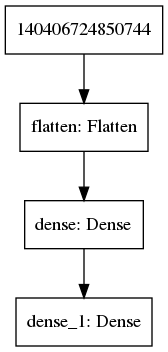
\includegraphics[width=0.3\textwidth]{../images/model-v1}
  \caption{Configuración de capas de la primera versión}
  \label{fig:capas-v1}
\end{figure}

\bigskip

Con esta configuración tan simple pude obtener un porcentaje de acierto sobre el conjunto de entrenamiento del \textbf{99.8\%} y un \textbf{97.62\%} sobre el conjunto de prueba, que me pareció un resultado más que aceptable para una primera versión. Los resultados de esta versión pueden verse detallados en profundidad en el siguiente capítulo.

\bigskip

La ejecución de esta versión duró un poco más que la primera (~300 segundos frente a los solamente ~20 segundos de la primera), así que aunque al principio me planteé usar algún servicio PaaS\footnote{Platform as a Service} como \textit{Amazon Web Services} para ejecutar la práctica, finalmente decidí que debido a su coste y a que los tiempos no eran excesivamente altos podía seguir ejecutándola en mi ordenador personal.

\bigskip

El enlace de esta versión en el repositorio es \url{https://github.com/gomezportillo/mnist/tree/v1.0}.


\section{Segunda versión}

Como ya tenía configurado el entorno de desarrollo y sabía cómo trabajar con el framework elegido, en la segunda versión pude navegar tranquilamente por la API de Keras\footnote{\url{https://keras.io/}} para conocer y entender todas las funciones y parámetros que tiene.

\bigskip

Al final realicé una configuración de 5 capas, usando un modelo secuencial con 15 épocas de entrenamiento.

\bigskip

\begin{itemize}
  \item La primera capa, llamada  \textit{Conv2D}, es una capa convolutiva con la función de activación de rectificación lineal y una ventana convolutiva de 3x3.
  \item La segunda capa, llamada \textit{MaxPooling2D}, es una capa de operación de agrupación máxima con un tamaño de pool de 2x2.
  \item La tercera capa, llamada \textit{Dropout}, descarta el 25\% de las neuronas aleatoriamente para evitar problemas de sobreapendizaje en la fase de entrenamiento.
  \item La cuarta capa, llamada \textit{Flatten}, convierte los datos de entrada de una matriz bidimensional de 28x28 a un vector unidimensional para que puedan ser procesados por capas totalmente conectadas.
  \item La quinta capa, llamada \textit{Dropout}, tiene un número de nodos igual al número de clases del modelo, del 0 al 9, con la función de activación \textit{softmax} para poder realizar predicciones más adelante.
\end{itemize}

\bigskip

La imagen \ref{fig:capas-v2} refleja la configuración de capas utilizada.

\bigskip

\begin{figure}[H]
  \centering
  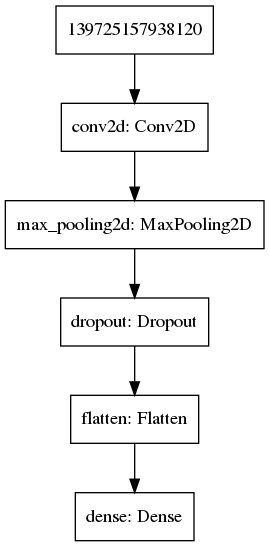
\includegraphics[width=0.45\textwidth]{../images/model-v2}
  \caption{Configuración de capas de la segunda versión}
  \label{fig:capas-v2}
\end{figure}

\bigskip

Con esta configuración, algo más compleja, ya que usa capas convolutivas e intenta evitar el sobreaprendizaje de la red usando funciones dropout, fue posible obtener un porcentaje de acierto sobre el conjunto de entrenamiento de un \textbf{99.27\%} y un \textbf{98.22\%} sobre el conjunto de prueba.

\bigskip

Me pareció interesante que, comparado con la versión anterior, normalmente obtenía resultados algo peores en el conjunto de entrenamiento pero casi un 1\% mejores en el conjunto de prueba, lo que achaqué a que había solucionado los problemas de sobreaprendizaje.

\bigskip

El enlace de esta versión en el repositorio es \url{https://github.com/gomezportillo/mnist/tree/v2.0}.

\section{Tercera versión}

Por último, en la tercera versión del proyecto necesitaba un porcentaje de aciertos lo más cercano al 100\% posible tanto en el conjunto de entrenamiento como en el prueba.

\bigskip

El resultado final fue una configuración de 9 capas, usando un modelo secuencial con 20 épocas de entrenamiento. Como ya había resuelto el problema del sobreaprendizaje pude usar más épocas de entrenamiento que en las versiones anteriores.

\bigskip

\begin{itemize}
  \item La primera capa es una capa convolutiva llamada \textit{Conv2D} con una función de activación de rectificación lineal, 32 mapas característicos y una ventana convolutiva de 4x4.
  \item La segunda capa es una capa convolutiva llamada \textit{Conv2D} con la función de activación de rectificación lineal y una ventana convolutiva de 3x3.
  \item La tercera capa, llamada \textit{MaxPooling2D}, es una capa de operación de agrupación máxima con un tamaño de pool de 2x2.
  \item La cuarta capa, llamada \textit{Dropout}, descarta el 20\% de las neuronas aleatoriamente para evitar problemas de sobreapendizaje en la fase de entrenamiento.
  \item La quinta capa, llamada \textit{Flatten}, convierte los datos de la matriz bidimensional en un vector lineal para que la sexta capa pueda ser una capa completamente conectada.
  \item La sexta capa, llamada \textit{Dense}, es una capa completamente conectada con 248 neuronas y función de activación de rectificación lineal.
  \item La séptima capa, llamada \textit{Dense}, es una capa completamente conectada con 124 neuronas (la mitad que la anterior) y función de activación de rectificación lineal.
  \item La octava capa, llamada \textit{Dropout}, vuelve a descartar el 40\% de las neuronas aleatoriamente.
  \item La novena capa, llamada \textit{Dense}, es la capa de salida, con 10 neuronas (una por cada clase) y una función de activación \textit{softmax} para poder realizar predicciones probabilísticas más adelante.
\end{itemize}

\bigskip

La imagen  \ref{fig:capas-v3} refleja la configuración final de capas utilizada.

\bigskip

\begin{figure}[H]
  \centering
  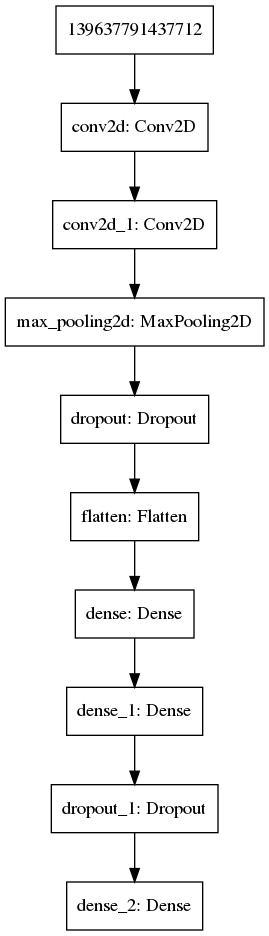
\includegraphics[width=0.5\textwidth]{../images/model-v3}
  \caption{Configuración de capas de la tercera versión}
  \label{fig:capas-v3}
\end{figure}

\bigskip

Con esta configuración pude obtener un porcentaje de aciertos sobre el conjunto de prueba de un \textbf{99.91\%} y un \textbf{99.15\%} sobre el conjunto de prueba.

El enlace de esta versión en el repositorio es \url{https://github.com/gomezportillo/mnist/tree/v3.0}.

\chapter{Resultados}
\label{chap:res}

A continuación se presentan los resultados detallados de las diferentes versiones del proyecto.

\bigskip

\section{Primera versión}

Tras ejecutar la primera versión, cuya fase de entrenamiento duró \textbf{22.2 segundos}, obtuve los siguientes resultados, formateados en la tabla \ref{tab:v1}. La columna \textit{Época} indica a qué época del entrenamiento hacen referencia los resultados, la columna \textit{Loss} es un valor escalar que intentamos reducir a 0 y la columna \textit{Acierto} indica el porcentaje de aciertos que se han obtenido.

\bigskip

\begin{table}[H]
  \centering
  \begin{tabular}{|l|l|l||l|l|l|}
    \hline
    \textbf{Época} & \textbf{Loss} & \textbf{Acierto} & \textbf{Época} & \textbf{Loss} & \textbf{Acierto} \\
    \hline
    1     & 0.3603 & 0.9007  & 11    & 0.0271 & 0.9927  \\
    2     & 0.1674 & 0.9526  & 12    & 0.0240 & 0.9939  \\
    3     & 0.1205 & 0.9656  & 13    & 0.0209 & 0.9946  \\
    4     & 0.0929 & 0.9736  & 14    & 0.0174 & 0.9958  \\
    5     & 0.0750 & 0.9784  & 15    & 0.0149 & 0.9965  \\
    6     & 0.0622 & 0.9819  &       &        &         \\
    7     & 0.0524 & 0.9853  &       &        &         \\
    8     & 0.0439 & 0.9877  &       &        &         \\
    9     & 0.0375 & 0.9895  &       &        &         \\
    10    & 0.0326 & 0.9911  &       &        &         \\
    \hline
  \end{tabular}
  \label{tab:v1}
  \caption{Resultados de la fase de entrenamiento de la primera versión}
\end{table}

\bigskip

El gráfico \ref{fig:res-v1} refleja los datos de la tabla anterior.

\bigskip

\begin{figure}[H]
  \centering
  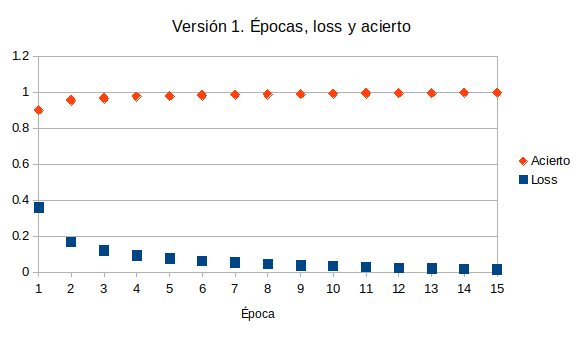
\includegraphics[width=1\textwidth]{../images/results-v1}
  \caption{Gráfico de la fase de entrenamiento de la primera versión}
  \label{fig:res-v1}
\end{figure}

\bigskip

Tras la fase de entrenamiento evalué el modelo, primero con el conjunto de entrenamiento y luego con el conjunto de prueba, y obtuve los siguientes resultados, que pueden verse en la tabla inferior.

\bigskip

\begin{table}[H]
  \centering
  \begin{tabular}{|l|l|l|}
    \hline
    \textbf{Conjunto} & \textbf{Loss} & \textbf{Acierto} \\
    \hline
    Entrenamiento & 0.01141 & 99.80500\%  \\
    Prueba        & 0.07754 & 97.62000\%  \\
    \hline
  \end{tabular}
  \label{tab:results-v1}
  \caption{Resultados de la primera versión dependiendo del conjunto}
\end{table}

\bigskip

A modo de ejemplo, se ha incluido la salida de la consola tras ejecutar esta versión, que puede comprobarse en el  anexo \ref{sec:v1-output}.

\section{Segunda versión}

Tas ejecutar la segunda versión, cuya fase de entrenamiento duró \textbf{309.8 segundos}, obtuve los siguientes resultados.

\bigskip

\begin{table}[H]
  \centering
  \begin{tabular}{|l|l|l||l|l|l|}
    \hline
    \textbf{Época} & \textbf{Loss} & \textbf{Acierto} & \textbf{Época} & \textbf{Loss} & \textbf{Acierto} \\
    \hline
    1                       & 0.3648 & 0.8989 & 11 & 0.0497 & 0.9845 \\
    2                       & 0.1361 & 0.9618 & 12 & 0.0478 & 0.9854 \\
    3                       & 0.1361 & 0.9712 & 13 & 0.0455 & 0.9860 \\
    4                       & 0.0847 & 0.9757 & 14 & 0.0410 & 0.9872 \\
    5                       & 0.0759 & 0.9773 & 15 & 0.0404 & 0.9874 \\
    6                       & 0.0691 & 0.9791 &    &        &        \\
    7                       & 0.0628 & 0.9815 &    &        &        \\
    8                       & 0.0599 & 0.9821 &    &        &        \\
    9                       & 0.0567 & 0.9830 &    &        &        \\
    10                      & 0.0522 & 0.9835 &    &        &        \\
    \hline
  \end{tabular}
  \label{tab:v2}
  \caption{Resultados de la fase de entrenamiento de la segunda versión}
\end{table}

\bigskip

El gráfico \ref{fig:res-v2} refleja los datos de la esta tabla.

\bigskip

\begin{figure}[H]
  \centering
  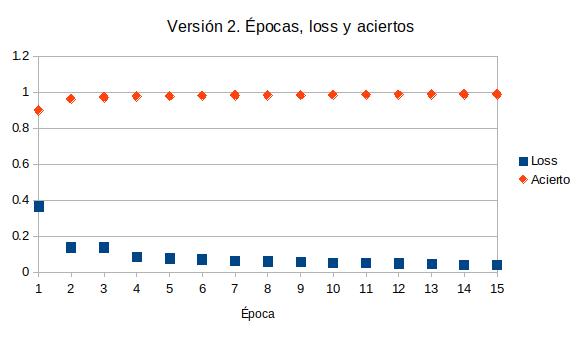
\includegraphics[width=1\textwidth]{../images/results-v2}
  \caption{Gráfico de la fase de entrenamiento de la segunda versión}
  \label{fig:res-v2}
\end{figure}

\bigskip

Tras la fase de entrenamiento evalué el modelo, primero con el conjunto de entrenamiento y luego con el conjunto de prueba, y obtuve los siguientes resultados.

\bigskip

\begin{table}[H]
  \centering
  \begin{tabular}{|l|l|l|}
    \hline
    \textbf{Conjunto} & \textbf{Loss} & \textbf{Acierto} \\
    \hline
    Entrenamiento & 0.02590 & 99.27000\%  \\
    Prueba        & 0.05184 & 98.22000\%  \\
    \hline
  \end{tabular}
  \label{tab:results-v2}
  \caption{Resultados de la segunda versión dependiendo del conjunto}
\end{table}

\bigskip

\section{Tercera versión}

Tas ejecutar la tercera versión, cuya fase de entrenamiento duró 309.8 segundos, obtuve los siguientes resultados.

\bigskip

\begin{table}[H]
  \centering
  \begin{tabular}{|l|l|l||l|l|l|}
    \hline
    \textbf{Época} & \textbf{Loss} & \textbf{Acierto} & \textbf{Época} & \textbf{Loss} & \textbf{Acierto} \\
    \hline
    1                       & 0.1970 & 0.9389 & 11 & 0.0093 & 0.9971 \\
    2                       & 0.0560 & 0.9831 & 12 & 0.0088 & 0.9973 \\
    3                       & 0.0385 & 0.9882 & 13 & 0.0074 & 0.9978 \\
    4                       & 0.0288 & 0.9909 & 14 & 0.0078 & 0.9975 \\
    5                       & 0.0227 & 0.9934 & 15 & 0.0055 & 0.9983 \\
    6                       & 0.0198 & 0.9940 & 16 & 0.0076 & 0.9977 \\
    7                       & 0.0160 & 0.9952 & 17 & 0.0060 & 0.9983 \\
    8                       & 0.0130 & 0.9957 & 18 & 0.0064 & 0.9980 \\
    9                       & 0.0114 & 0.9964 & 19 & 0.0039 & 0.9988 \\
    \hline
  \end{tabular}
  \label{tab:v3}
  \caption{Resultados de la fase de entrenamiento de la tercera versión}
\end{table}

\bigskip

El gráfico \ref{fig:res-v3} refleja los datos de la esta tabla.

\bigskip

Tras la fase de entrenamiento evalué el modelo, primero con el conjunto de entrenamiento y luego con el conjunto de prueba, y obtuve los siguientes resultados.

\bigskip

\begin{table}[H]
  \centering
  \begin{tabular}{|l|l|l|}
    \hline
    \textbf{Conjunto} & \textbf{Loss} & \textbf{Acierto} \\
    \hline
    Entrenamiento & 0.00237 & 99.90167\%  \\
    Prueba        & 0.04271 & 99.15000\%  \\
    \hline
  \end{tabular}
  \label{tab:results-v3}
  \caption{Resultados de la tercera versión dependiendo del conjunto}
\end{table}

\bigskip

\begin{figure}[H]
  \centering
  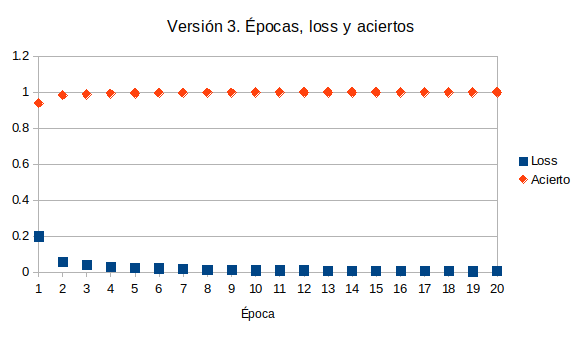
\includegraphics[width=1\textwidth]{../images/results-v3}
  \caption{Gráfico de la fase de entrenamiento de la tercera versión}
  \label{fig:res-v3}
\end{figure}

\bigskip

Por lo tanto, el \textbf{resultado final} del proyecto sobre el conjunto de prueba es de un 99.15\%, lo que supone tan solo un \textbf{0.85\% de fallos sobre los 10,000 números manuscritos}, o lo que es lo mismo, 85 errores.

\chapter{Conclusiones}
\label{chap:concl}

Las redes neuronales son un campo muy profundo y, aunque esta práctica solo me ha servido como introducción a él, me alegro mucho de haberla realizado. Sé que, tarde o temprano, en mi futura vida laboral tendré que realizar un proyecto basado en redes neuronales y esta práctica me servirá para recordar conceptos y tener un punto de partida. 

\bigskip

Creo que ha sido un modo muy bueno de aplicar los términos y conceptos estudiados en teoría, viendo cómo la práctica avanzaba a través de sus diferentes versiones, aunque al haberlo ejecutado en local los tiempos de espera hayan sido, sobre todo hacia el final de la práctica, bastante elevados.

\bigskip

Personalmente estoy muy contento con los resultados obtenidos. He pasado de conocer las redes neuronales de un modo teórico a configurar y usar un framework de desarrollo de deep learning y obtener unos resultados muy cercanos a un 100\% de acierto. 
\chapter{Referencias}
\label{chap:refer}

\begin{itemize}
  \item \url{https://www.tensorflow.org/tutorials/keras/basic_classification}
  \item \url{https://www.tensorflow.org/guide/keras}
  \item \url{https://github.com/erseco/ugr_inteligencia_computacional}
  \item \url{https://nextjournal.com/gkoehler/digit-recognition-with-keras}
  \item \url{https://github.com/keras-team/keras/blob/master/examples/mnist_cnn.py}
  \item \url{http://www.machinelearningtutorial.net/2016/12/24/python-keras-mnist/}
  \item \url{https://pythonprogramming.net/mnist-python-playing-neural-network-tensorflow/}
  \item \url{https://mxnet.incubator.apache.org/tutorials/python/mnist.html}
  \item \url{https://github.com/keras-team/keras/blob/master/examples/mnist_cnn.py}
  \item \url{https://www.kaggle.com/moghazy/guide-to-cnns-with-data-augmentation-keras}
\end{itemize}

\chapter{Anexos}
\label{chap:anexos}

\section{Anexo 1. Salida de la consola tras ejecutar la primera versión}
\label{sec:v1-output}

\bigskip

\begin{lstlisting}[language=bash]
/usr/bin/python3 src/mnist.py
Using TensorFlow backend.
Using TensorFlow v1.12.0
The number of occuranc of each number in the train set is {0: 5923, 1: 6742, 2: 5958, 3: 6131, 4: 5842, 5: 5421, 6: 5918, 7: 6265, 8: 5851, 9: 5949}

The number of occuranc of each number in the test set is {0: 980, 1: 1135, 2: 1032, 3: 1010, 4: 982, 5: 892, 6: 958, 7: 1028, 8: 974, 9: 1009}

Train on 60000 samples, validate on 60000 samples
Epoch 1/15
2018-11-22 23:14:01.439601: I tensorflow/core/platform/cpu_feature_guard.cc:141] Your CPU supports instructions that this TensorFlow binary was not compiled to use: AVX2 FMA
60000/60000 [==============================] - 2s 27us/step - loss: 0.3603 - acc: 0.9007 - val_loss: 0.1898 - val_acc: 0.9472
Epoch 2/15
60000/60000 [==============================] - 1s 24us/step - loss: 0.1674 - acc: 0.9526 - val_loss: 0.1290 - val_acc: 0.9639
Epoch 3/15
60000/60000 [==============================] - 1s 25us/step - loss: 0.1205 - acc: 0.9656 - val_loss: 0.0996 - val_acc: 0.9711
Epoch 4/15
60000/60000 [==============================] - 1s 25us/step - loss: 0.0929 - acc: 0.9736 - val_loss: 0.0774 - val_acc: 0.9777
Epoch 5/15
60000/60000 [==============================] - 1s 24us/step - loss: 0.0750 - acc: 0.9784 - val_loss: 0.0606 - val_acc: 0.9826
Epoch 6/15
60000/60000 [==============================] - 1s 24us/step - loss: 0.0622 - acc: 0.9819 - val_loss: 0.0499 - val_acc: 0.9866
Epoch 7/15
60000/60000 [==============================] - 1s 25us/step - loss: 0.0524 - acc: 0.9853 - val_loss: 0.0417 - val_acc: 0.9884
Epoch 8/15
60000/60000 [==============================] - 2s 25us/step - loss: 0.0439 - acc: 0.9877 - val_loss: 0.0369 - val_acc: 0.9902
Epoch 9/15
60000/60000 [==============================] - 1s 25us/step - loss: 0.0375 - acc: 0.9895 - val_loss: 0.0288 - val_acc: 0.9930
Epoch 10/15
60000/60000 [==============================] - 1s 24us/step - loss: 0.0326 - acc: 0.9911 - val_loss: 0.0243 - val_acc: 0.9942
Epoch 11/15
60000/60000 [==============================] - 1s 24us/step - loss: 0.0271 - acc: 0.9927 - val_loss: 0.0218 - val_acc: 0.9952
Epoch 12/15
60000/60000 [==============================] - 1s 24us/step - loss: 0.0240 - acc: 0.9939 - val_loss: 0.0168 - val_acc: 0.9963
Epoch 13/15
60000/60000 [==============================] - 2s 26us/step - loss: 0.0209 - acc: 0.9946 - val_loss: 0.0161 - val_acc: 0.9966
Epoch 14/15
60000/60000 [==============================] - 2s 26us/step - loss: 0.0174 - acc: 0.9958 - val_loss: 0.0128 - val_acc: 0.9973
Epoch 15/15
60000/60000 [==============================] - 2s 25us/step - loss: 0.0149 - acc: 0.9965 - val_loss: 0.0114 - val_acc: 0.9980
Training time: 22.613s
60000/60000 [==============================] - 1s 22us/step
Train loss: 0.01141
Train accuracy: 99.80500%
10000/10000 [==============================] - 0s 23us/step
Test loss: 0.07754
Test accuracy: 97.62000%

\end{lstlisting}

\newpage
\section{Anexo 2. Estructura de directorios del proyecto}

\bigskip

\begin{itemize}
  \item El direcotrio \textit{deliverables/} contiene los resultados de cada versión del proyecto.
  \item La carpeta \textit{doc/} contiene la documentación final y el guión de la práctica.
  \item Los archivo \textit{LICENSE} y \textit{README.txt} son archivos de configuración del repositorio.
  \item El archivo \textit{Makefile} sirve para instalar y ejecutar el proyecto.
  \item El archivo \textit{requirements.txt} contiene los nombres y las versiones de las librerías utilizadas en el proyecto, y es usado por la herramienta pip para instalarlas.
  \item El directorio \textit{src/} contiene los archivos de código fuente de la práctica.
  \begin{itemize}
    \item \textit{aux.py} contiene funciones auxiliares utilizados para renderizar las imágenes de la base de datos.
    \item \textit{mist\_functions.py} contiene las llamadas a la API de Keras envueltas en funciones personalizadas ya que, en un intento por aumentar la claridad y la mantenibilidad del proyecto, el archivo principal llama a estas funciones.
    \item \textit{mnist.py} es el archivo principal y contiene la inicialización de las librerías, la configuración de las capas de la red neuronal y las llamadas a las funciones de \textit{mnist\_functions.py}.
  \end{itemize}
\end{itemize}


\newpage
\section{Anexo 3. Código fuente de la práctica}

\subsection{mnist.py}

\begin{lstlisting}[language=python]
#!/usr/bin/python3
# -*- coding:utf-8 -*-

# TensorFlow and tf.keras
import tensorflow as tf
from tensorflow import keras
from keras import backend
print("Using TensorFlow v{}".format(tf.__version__))

#Local libraries
from aux import *
from mnist_functions import *

# Downloading MNIST dataset from keras
(train_images, train_labels), (test_images, test_labels) = keras.datasets.mnist.load_data()

# Getting unique values from labels, sorting them and storing
class_names = list(set(train_labels))
num_classes = len(class_names)
input_shape = (28, 28, 1) # 28x28 pixels, no z coordinate

# Printing how manny different numbers are in each set
print_unique_numbers('train', train_labels)
print_unique_numbers('test', test_labels)

# Prepocessing
## Normalising datasets before feeding to the neural network
train_images = train_images / 255.0
test_images = test_images / 255.0

train_images = train_images.reshape(train_images.shape[0], 28, 28, 1)
train_images = train_images.astype('float32')

test_images = test_images.reshape(test_images.shape[0], 28, 28, 1)
test_images = test_images.astype('float32')

## convert class vectors to binary class matrices
train_labels = keras.utils.to_categorical(train_labels, num_classes)
test_labels = keras.utils.to_categorical(test_labels, num_classes)

# Building the model
model = keras.Sequential()
model.add(keras.layers.Conv2D(32, kernel_size=(4, 4),
activation=tf.nn.relu,
input_shape=input_shape))
model.add(keras.layers.Conv2D(64, (3, 3), activation=tf.nn.relu))
model.add(keras.layers.MaxPooling2D(pool_size=(2, 2)))
model.add(keras.layers.Dropout(0.2))
model.add(keras.layers.Flatten())
model.add(keras.layers.Dense(248, activation=tf.nn.relu))
model.add(keras.layers.Dense(124, activation=tf.nn.relu))
model.add(keras.layers.Dropout(0.4))
model.add(keras.layers.Dense(num_classes, activation=tf.nn.softmax))

# Compiling the model
model.compile(optimizer=keras.optimizers.Adam(),
loss=keras.losses.categorical_crossentropy,
metrics=['accuracy'])

# Train the model with the train images
EPOCHS = 20

train_time_str = train_model(model, train_images, train_labels, EPOCHS)

# Evaluate the accuracy of the model with the train images
train_loss_str, train_acc_str = evaluate_model('Train', model, train_images, train_labels)

# Evaluate the accuracy of the model with the test images
test_loss_str, test_acc_str = evaluate_model('Test', model, test_images, test_labels)

# Save results
VERSION = 3
save_results(VERSION, train_time_str, train_loss_str, train_acc_str, test_loss_str, test_acc_str)

# Predicting the labels of all train images
predict_labels(VERSION, 'train', model, train_images)

# Predicting the labels of all test images
predict_labels(VERSION, 'test', model, test_images)

save_model_layers_to_file(VERSION, 'model.png', model)
\end{lstlisting}


\subsection{mist\_functions.py}

\begin{lstlisting}[language=python]
#!/usr/bin/python3
# -*- coding:utf-8 -*-

import time
import os
import numpy
from keras.utils import plot_model

def print_unique_numbers(TYPE, labels):
    unique, count= numpy.unique(labels, return_counts=True)
    print("The number of occurrence of each number in the {} set is {}\n".format(TYPE, dict (zip(unique, count))))


def train_model(model, images, labels, EPOCHS):
    start_time = time.time()

    model.fit(images, labels, epochs=EPOCHS, batch_size=128, validation_data=(images, labels))

    end_time = time.time()
    elapsed_time = end_time - start_time
    elapsed_time_str = "Training time: {:.3f}s".format(elapsed_time)
    print(elapsed_time_str)

    return elapsed_time_str

def evaluate_model(TYPE, model, images, labels):
    loss, acc = model.evaluate(images, labels)
    loss_str = '{0} loss: {1:.5f}'.format(TYPE, loss)
    acc_str = '{0} accuracy: {1:.5f}%'.format(TYPE, acc*100)
    print(loss_str)
    print(acc_str)

    return (loss_str, acc_str)

def save_results(VERSION, train_time, train_loss, train_acc, test_loss, test_acc):
    dir_name = 'deliverables/ver_{0}/'.format(VERSION)
    if not os.path.exists(dir_name):
        os.makedirs(dir_name)

    filename = dir_name + 'result.txt'
    with open(filename, 'w') as f_out:
        f_out.write(train_time + '\n')
        f_out.write(train_loss + '\n')
        f_out.write(train_acc + '\n')
        f_out.write(test_loss + '\n')
        f_out.write(test_acc + '\n')

def predict_labels(VERSION, TYPE, model, images):
    predictions = model.predict(images)
    assigned_labels = numpy.argmax(predictions, axis=-1)

    assert len(predictions) == len(images)

    filename = 'deliverables/ver_{0}/assigned_labels_{1}.txt'.format(VERSION, TYPE)
    with open(filename, 'w') as f_out:
        for label in assigned_labels:
            f_out.write(str(label))

    return assigned_labels

def save_model_layers_to_file(VERSION, name, model):
    filename = 'deliverables/ver_{0}/{1}'.format(VERSION, name)

    plot_model(model, to_file=filename)
\end{lstlisting}


\subsection{aux.py}

\begin{lstlisting}[language=python]
#!/usr/bin/python3
# -*- coding:utf-8 -*-

import matplotlib.pyplot as plt

def render_image(image):
    plt.figure()
    plt.imshow(image)
    plt.colorbar()
    plt.grid(False)
    plt.ylabel('Rendered image')
    plt.show()

def render_imagelist(images, labels, class_names):
    plt.figure(figsize=(10,10))
    for i in range(25):
        plt.subplot(5,5,i+1)
        plt.xticks([])
        plt.yticks([])
        plt.grid(False)
        plt.imshow(images[i], cmap=plt.cm.binary)
        plt.xlabel(class_names[labels[i]])
    plt.show()
\end{lstlisting}


\newpage \
\thispagestyle{empty}
\end{document}
